\chapter[Conclusion \&~Open Problems]{Conclusion \& Open Problems}
\label{ch:conclu-database}
\renewcommand\thefigure{\thechapter.\arabic{figure}}

\begin{chapterpresentation}
	\begin{abstract}
		\todo{}
	\end{abstract}
		
	\par\bigskip\bigskip
	\chaptertoc
\end{chapterpresentation}

\section{Minimization Problems}

Rather than closing the complexity gaps between our "$k$-ExpSpace" upper bounds
and the "ExpSpace" lower bounds in the decision problems
studied in \Cref{ch:minimization-CRPQ,ch:semantic-tree-width-CRPQ},
we believe that the most interesting questions "wrt" to minimization
are actually those related to \emph{structure}, and more precisely those that try to
connect the different notions of minimality together.

\conjAtomVariableMinimal*

\paragraph*{Minimization \& Trees.}
The question of whether the seminal results of \cite{CzerwinskiMartensNiewerthParys2018Minimization} could be lifted from "tree patterns"
to their encoding as "CRPQs" remain open.
\conjTreePatternsAsCRPQs*

On a similar note, an interesting question is whether two goals
("eg" the number of variables and the number of "atoms")
can be simultaneously minimized.
For "CQs", this is always the case by \Cref{prop:minimization-CQ}. However, this question
seems quite hard for "CRPQs", even on concrete examples.
We say that a "CRPQ" is ""forest-shaped"" if its underlying "directed graph"
is a "disjoint union" of "directed trees".
\begin{question}
	Is it the case that every "Boolean CRPQ" that is (1) "equivalent@@sem" to
	a "forest-shaped" "CRPQ" and (2) "equivalent@@sem" to a "CRPQ"
  with at most $k$ "atoms" is necessarily "equivalent@@sem" to a 
  "forest-shaped" "CRPQ" with at most $k$ "atoms"?
\end{question}
We conjecture the answer to this question to be yes, but we were unable to prove it:
we only managed to prove that, under these assumptions, the query
should be "equivalent@@sem" to a "forest-shaped" "CRPQ" with at most $2^k$ "atoms"
(\Cref{thm:charac-semantically-forest-shaped}).


\paragraph*{Maximal Under-Approximations.}
Both the result on "UCRPQ minimization" of \Cref{ch:minimization-CRPQ}
and of "semantic tree-width" minimization of \Cref{ch:semantic-tree-width-CRPQ} 
rely on the existence---and computability---of "maximal under-approximations".
In the first case, the target class consists of finitely many graphs (\Cref{lemma:approximation-for-finclass}), but in the second case,
it is infinite (\Cref{lemma:bound_size_refinements}): as such the proof is significantly harder.
Having the remarkable genericity of \Cref{prop:minimization-CQ} in mind,
we could only hope to be able to capture 
both \Cref{lemma:approximation-for-finclass,lemma:bound_size_refinements}.

\begin{question}
	Given a class $\+C$ of "graphs@@dir" that is "closed under minors",
	do "maximal under-approximations" by "UC(2)RPQs" over $\+C$ always exist?
	If so, are they computable?
\end{question}

\section{Profinite Databases}

\begin{marginfigure}[8em]
	\centering
	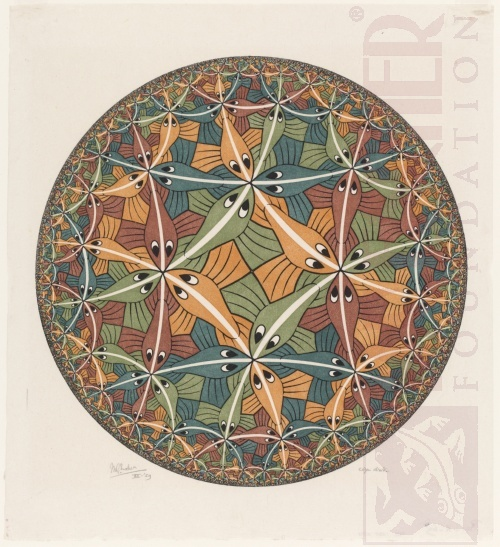
\includegraphics[width=\linewidth]{fig/escher/CL3.jpg}
	\caption{\href{https://mcescher.com/gallery/symmetry/\#iLightbox[gallery\_image_1]/12}{\emph{Circle Limit III}}, M. C. Escher, \textcopyright~The M.C. Escher Company.}
\end{marginfigure}
As we have seen in \Cref{sec:prelim-db-relational}, "duality"---namely the existence of
a dual "isomorphism" between queries and models---provides a remarkable framework to
study "conjunctive queries". For the more complex language of "conjunctive regular path queries",
however, this isomorphism fails, making static analysis much harder.
We thought that part of the enjoyable properties of "conjunctive queries"
could be recovered for "CRPQs" by considering the notion of "profinite databases".
In short, a \AP""profinite database"" consists of, a ``projective system'' of finite "graph databases",
"ie" an $\omega$-sequence of "homomorphisms"
\[
	\?G_0 \cohomto \?G_1 \cohomto \dotsc \cohomto \?G_n \cohomto \?G_{n+1} \cohomto \dotsc
\]
that we denote by $\varprojlim\limits_{n\in\N} \?G_n$.

\smallskip

A typical example of such a system can be obtained as follows:
just like we did in \Cref{sec:prelim-db-relational},
we let $\?C_n$ ($n\in\Np$) denote the directed cycle with domain $\ZnZ{n}$
and with an edge from $i$ to $j$ "iff" $i+1 = j$, see \Cref{fig:conclu-db-cycles}.
Recall that $\?C_n \homto \?C_m$ "iff" $n$ is a multiple of $m$.
In particular, we have
\[
	\?C_1 \cohomto \?C_2 \cohomto \dotsc \cohomto \?C_{2^n} \cohomto \?C_{2^{n+1}} \cohomto \dotsc.
\]
\begin{figure}
	\centering
	\begin{tikzpicture}
		\foreach \i in {0,...,5} {
			\pgfmathtruncatemacro\j{mod(\i, 3)}
			\node[vertex, draw=c\j, fill=c\j, fill opacity=.4] (s\i) at (\i*360/6: 1.2cm) {};
		}
		\foreach \i in {0,...,5} {
			\pgfmathtruncatemacro\ip{mod(\i+1, 6)}
			\draw[edge] (s\i) to (s\ip);
		}

		\foreach \i in {0,1,2} {
			\node[vertex, draw=c\i, fill=c\i, fill opacity=.4] (t\i) at ($(\i*360/3: .9cm)+(5, 0)$) {};
		}
		\foreach \i in {0,1,2} {
			\pgfmathtruncatemacro\ip{mod(\i+1, 3)}
			\draw[edge] (t\i) to (t\ip);
		}
	\end{tikzpicture}
	\caption{\AP\label{fig:conclu-db-cycles} The "graphs@@dir" $\?C_6$
	(left) and $\?C_3$ (right) and a "homomorphism" from the former
	to the latter, described by colour coding. (Replica of \Cref{fig:prelim-db-cycles}.)}
\end{figure}

The crucial point is that projective system have a natural semantics:
we define the semantics of \[\varprojlim\limits_{n\in\N} \?G_n\]
as the set of points that above some element of this sequence,
"ie" as
\[
	\?H \vDash \semFO{\varprojlim\limits_{n\in\N} \?G_n}
	\quad\text{when}\quad
	\exists n.\; \?G_n \homto \?H.
\]
For instance
\[\varprojlim\limits_{n\in\N} \?C_{2^n}\] has a simple
semantical interpretation:
letting $\?G$ be a "graph database", for any $n\in\N$, we get that $\?C_{2^n} \homto \?G$
if, and only if, $\?G$ contains a "directed cycle" of length $2^n$.
And so, there exists $n\in\N$ "st" $\?C_{2^n} \homto \?G$ if, and only if, $\?G$ contains
a "directed cycle" whose length is a power of 2.
In fact the true definition of projective system allows the sequence to
be indexed by a directed set rather than $\N$: in the case we would obtain
an object \[\varprojlim\limits_{n\in\tup{\Np,\mid}} \?C_{n},\] where we order $\Np$ by divisibility,
and whose semantics is ``the database contains a directed cycle''!

\paragraph{How Profinite Databases Arise.}
Profinite models naturally arise
by considering Stone duality. Roughly, Stone duality is a theory that,
starting from a logic and its models, adds new idealized/abstract models which
are necessary to make the theory compact, well-behaved and nicely describable.
For instance, applied to first-order logic over all structures,
this construction does nothing! This is precisely because this logic is already
\href{https://en.wikipedia.org/wiki/Compactness\_theorem}{compact}.
On the other hand, when applied to "regular languages" of finite words,
we obtained profinite words, which are exactly the models needed to describe
"pseudovarieties of monoids"! We refer the reader to \cite{GehrkeGool2024Topological}
for a not so short survey of the topic.

Second, "profinite databases" naturally appear when dealing with the semantics
of "CRPQs".%
\footnote{They actually are at the heart of
the proof of \Cref{thm:charac-semantically-forest-shaped}!}
Indeed, let $\gamma()$ and $\delta()$ be "CRPQs",
and assume that $\gamma() \semequiv \delta()$. Over "CQs", it would mean that
their "core@@CQ" are "isomorphic" (by \Cref{prop:equiv-core-isomorphic} and "duality"),
but over "CRPQs", we do not have such a nice characterization.
However, pick a "canonical database" $\?G_0 \cdb \gamma$. From the
fact that $\gamma \contained \delta$, we get the existence of $\?D_0 \cdb \delta$
"st" $\?G_0 \cohomto \?D_0$. In turn, using the converse "containment" $\delta \contained \gamma$,
we get that there exists $\?G_1 \cdb \gamma_1$ "st" $\?D_0 \cohomto \?G_1$. By induction,
we obtain an infinite sequence
\[
	\?G_0 \cohomto \?D_0 \cohomto \dotsc. \cohomto \?G_n \cohomto \?D_n \cohomto
	\?G_{n+1} \cohomto \?D_{n+1} \cohomto \dotsc.
\]
In other words, we get that the "profinite databases"
\[\varprojlim_{n\in\N} \?G_{n}
\quad\text{and}\quad
\varprojlim_{n\in\N} \?D_{n}\]
are "semantically equivalent"!

\begin{figure}
	\centering
	\begin{tikzpicture}[
		font=\footnotesize,
		every node/.style={inner sep=0pt,outer sep=0pt}
	]
		\begin{luacode}
-- parameters to tweak
-- nb of nodes in the lattice
width = 17 -- half-width
height = 17 -- half-height
-- height and width (in cm) of the tikzpicture
display_width = 11
display_height = 11
-- decay rates 
x_opacity_decay = 0.5
y_opacity_decay = 1.5
pos_decay = 1.6

cdb_x = 0
cdb_y = 0

dx = display_width / (2 * width)
dy = display_height / (2 * height)

function grid_to_picture_x(x)
	-- returns the position in the picture from the coordinates in the grid
	return x * dx * (math.abs(x)/width)^(pos_decay-1)
end 
function grid_to_picture_y(y)
	-- returns the position in the picture from the coordinates in the grid
	return y * dy * (math.abs(y)/height)^(pos_decay-1)
end

function is_part_of_grid(x,y)
	in_square = x >= -width and x <= width and y >= -height and y <= height
	in_check = (x+y)%2 ~= 0
	in_diamond = math.abs(x) <= height - math.abs(y)
	return in_square and in_check and in_diamond
end

function is_above(x1,y1,x2,y2) -- check if (x1,y1) is above (x2,y2)
	if y1 < y2 then
		return false
	end
	delta_y = y1 - y2 -- >= 0
	delta_x = math.abs(x2 - x1)
	return (delta_x <= delta_y)
end

function get_color(x,y)
	if is_above(x, y, cdb_x, cdb_y) then
		return "c1"
	else
		return "black" 
	end
end

function process_opacity(x)
	return 1/(1+math.exp(2.5-20*x))
end

function get_opacity(x,y)
	if y == 0 then
		return 0
	elseif math.abs(y) == height then
		return process_opacity(1)
	elseif math.abs(y) == 1 and math.abs(x) < width-1 then
		return process_opacity(0)
	elseif math.abs(x) == 1 and math.abs(y) < height-1 then
		y_opac = (math.abs(y/3)/height)^y_opacity_decay
		return process_opacity(y_opac)
	elseif math.abs(x) == 0 and math.abs(y) < height-1 then
		y_opac = (math.abs(y/4)/height)^y_opacity_decay
		return process_opacity(y_opac)
	else
		x_opac = (math.abs(x)/width)^x_opacity_decay
		y_opac = (math.abs(y)/height)^y_opacity_decay
		return process_opacity(x_opac * y_opac)
	end
end

function get_scale(x,y)
	return 2*get_opacity(x,y)^0.3
end

function get_edge_color(x1,y1,x2,y2)
	c1 = get_color(x1,y1)
	c2 = get_color(x2,y2)
	if c1 == c2 then
		return c1
	elseif c1 ~= "black" and c2 ~= "black" then
		return c1
	else
		return "black"
	end
end

function get_edge_opacity(x1,y1,x2,y2)
	o1 = get_opacity(x1,y1)
	o2 = get_opacity(x2,y2)
	return math.min(o1,o2)
end

-- define coordinates
for x = -width,width do
	for y = -height,height do
		if is_part_of_grid(x,y) then
			tex.print(string.format("\\coordinate (%i %i) at (%.4f, %.4f) {};", x, y, grid_to_picture_x(x), grid_to_picture_y(y)))
		end
	end 
end 
-- draw edges
for x = -width,width do
	for y = -height,height do
		if is_part_of_grid(x,y) then
			above = {{x-1,y+1}, {x+1, y+1}}
			for _, coord in ipairs(above) do 
				x2, y2 = coord[1], coord[2]
				if is_part_of_grid(x2,y2) then
					tex.print(string.format("\\draw[color=%s, opacity=%.4f] (%i %i) to[-] (%i %i);", get_edge_color(x,y,x2,y2), get_edge_opacity(x,y,x2,y2), x, y, x2, y2))
				end
			end
		end
	end 
end 
-- draw grid
for x = -width,width do
	for y = -height,height do
		if is_part_of_grid(x,y) then
			-- white background
			tex.print(string.format("\\node[circle,fill=white, minimum size=%.4f pt] at (%i %i) {};", get_scale(x,y), x, y))
			-- proper colour
			tex.print(string.format("\\node[circle,fill=%s, minimum size=%.4f pt, opacity=%.4f] at (%i %i) {};", get_color(x,y), get_scale(x,y), get_opacity(x,y), x, y))
		end
	end 
end 

\end{luacode}
\begin{luacode}
		function bloop(x,y)
			tex.print(string.format("\\node[circle,fill=white, minimum size=%.4f pt] at (%i %i) {};", get_scale(x,y), x, y))
			-- proper colour
			tex.print(string.format("\\node[circle,fill=%s, minimum size=%.4f pt, opacity=%.4f] at (%i %i) {};", "cOrange", 2.5*get_scale(x,y), get_opacity(x,y), x, y))
		end
		bloop(-1,0)
		bloop(0,1)
		bloop(-1,2)
		bloop(0,3)
		bloop(-1,4)
		bloop(-2,5)
		bloop(-3,6)
		bloop(-4,7)
		bloop(-3,8)
		bloop(-4,9)
		bloop(-5,10)
\end{luacode}
	\draw[thick, cOrange] (-5 10) to (-4 9) to (-3 8)
		to (-4 7) to (-3 6) to (-2 5) to (-1 4) to (0 3) to (-1 2) to (0 1) to (-1 0);
	\fill[white, path fading=myfading, fill opacity=.4] (0,0) circle[radius=1cm];
	\fill[white, path fading=myfading, fill opacity=.2] (0,0) circle[radius=.4cm];

	\end{tikzpicture}
	\caption{\AP\label{fig:poset-reldb-profinite}
	Semantics of a "query@@sem" that does admit a "hom-minimal" model
	(in yellow),
	together with a "profinite database" built out of its models
	in an effort to lift the opaque veil of the infinite structure of the distributive lattice
	of "graph databases" (in orange).
	}
\end{figure}

\paragraph{What Profinite Databases Could Help Us Achieve.}
In the previous chapters, we presented two results that where conditional
to the existence of "hom-minimal expansions":
\begin{itemize}
	\item the "semantical structure theorem" (\Cref{thm:structure-theorem}), which
		provides lower bounds on the complexity required to express a "CRPQ"---and which is,
		to out knowledge, actually the only result of this form for "CRPQs";
	\item a very partial generalization of "Grohe's theorem" to
		"finitely-redundant" Boolean "UC2RPQs" (\Cref{thm:tractability-finred}).
\end{itemize}
However, a very simple "CRPQ" such as $\gamma() \defeq x \atom{\A^*} x$,
expressing that the "database@@graph" contains "directed cycle" no do not
have "hom-minimal expansions", but it does have a "hom-minimal" 
"profinite database", which is \[\varprojlim\limits_{n\in\tup{\Np,\mid}} \?C_{n}.\]
More generally, by Zorn's lemma, every "CRPQ" admits at least 
one "hom-minimal" "profinite database", see \Cref{fig:poset-reldb-profinite}!

\begin{question}
	Can we generalize \Cref{thm:structure-theorem,thm:tractability-finred}
	to handle "hom-minimal" "profinite databases" rather than
	"hom-minimal" "finite databases"?
\end{question}

A positive answer to this question would provide a necessary and sufficient condition
on all "CRPQs" to be expressibly by simple "CRPQs", and might
lead to a characterization of tractable classes of "CRPQs"---which are results we can only dream of
given our current knowledge.

\quFPTtractability*

\begin{marginfigure}[-10em]
	\centering
	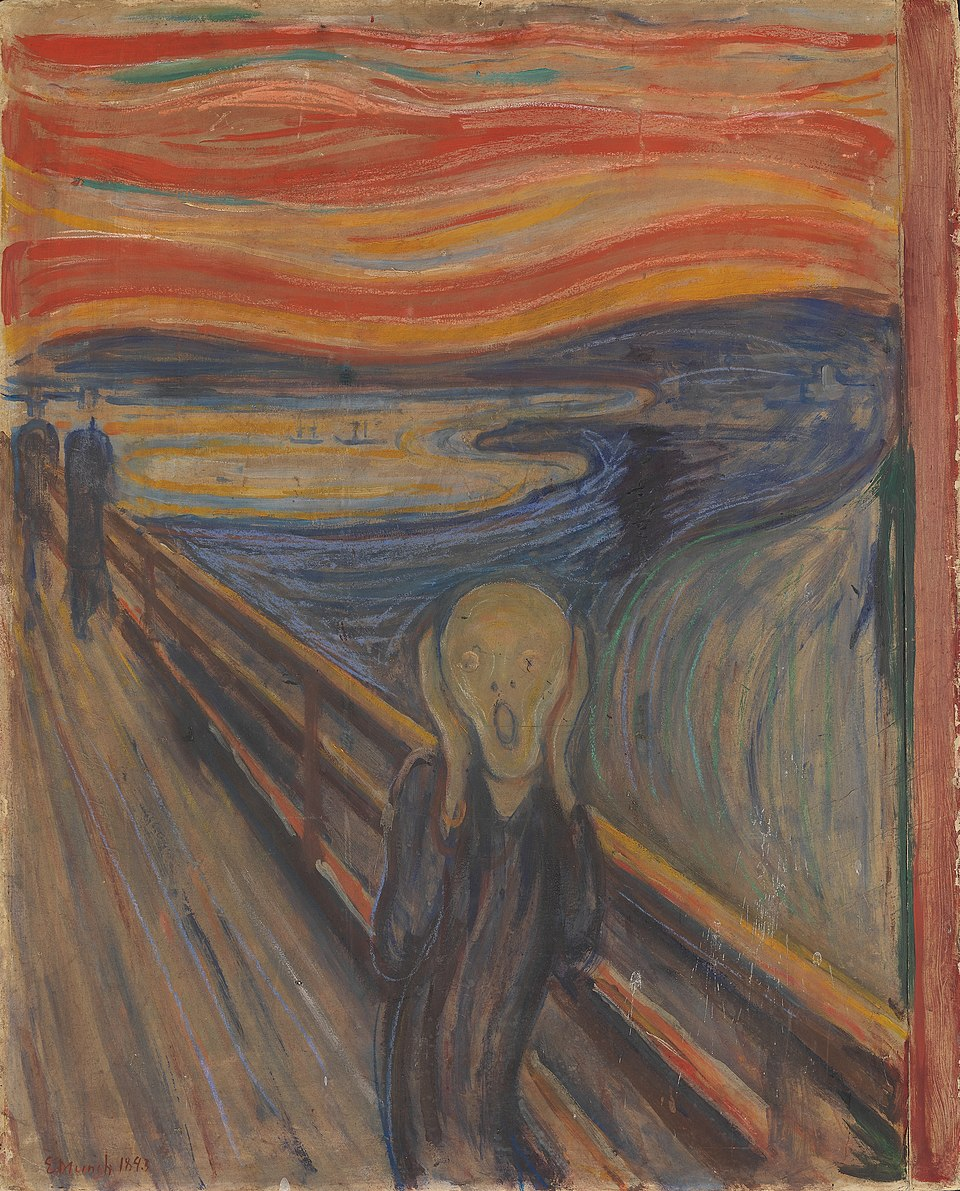
\includegraphics[width=\linewidth]{fig/Munch.jpg}
	\caption{
		When your Ph.D. student talks about
		the Stone dual space of the Heyting algebra of "conjunctive queries" for the forth
		time this month.
		\href{https://commons.wikimedia.org/wiki/File:Edvard\_Munch,\_1893,\_The_Scream,\_oil,\_tempera\_and\_pastel\_on\_cardboard,\_91\_x\_73\_cm,\_National\_Gallery\_of\_Norway.jpg}{\emph{Skrik}},
		by Edvard Munch.
	}
\end{marginfigure}
One the positive side, we managed to prove---in an unpublished work with Sam van Gool---that
the Stone dual of the Heyting algebra of "conjunctive queries" is isomorphic
to the space of "profinite databases", which seems to point towards the fact
that "profinite databases" are natural objects.

On the negative side, we do not know what to do with this result…
One of the main difficulties however is to find a reasonable definition for the notion of
``$\+C$-profinite databases''. We would like this notion to be defined at least whenever $\+C$ is a "minor-closed" "class of CRPQs", and intuitively $\+C$-profinite databases should
generalize the $\+C$-finite databases.
For instance, for "tree-width", we might have that "homomorphisms"
\[
	\?G \cohomto \?D \cohomto \?G'
\]
where $\?G$ and $\?G'$ have "tree-width" at most $k$,
but where $\?D$ is nowhere having "semantic tree-width" at most $k$…
More abstractly: "homomorphisms" do not interact that well with the notion of "minor".%
\footnote{This contrasts with the fact that "minor-closed classes" are closed under taking "cores".}

\clearpage
\begin{subappendices}
	\section{Tree-Like Queries}

\begin{hypothesis}
	 In this section, all "CRPQs" are assumed to be positive, meaning
	that no language can contain the empty word.
\end{hypothesis}

\subsection{Forest-Shaped and DAG-Shaped Queries}

We say that a CRPQ is \AP""semantically forest-shaped"" if it is
"semantically equivalent" to a CRPQ which is "forest-shaped".

Say that a CRPQ is \AP""DAG-shaped"" if its underlying directed multigraph
is a DAG---parallel edges are allowed, not self loops. If $\delta$ is "DAG-shaped",
define its \AP""unfolding"", denoted by \AP$\intro*\Unfold(\delta)$, as the following "CRPQ":
\begin{itemize}
	\item its variables are exactly labelled path of $\delta$
	of the form $x_0 \atom{L_1} \cdots \atom{L_n} x_n$ with $n\in \N$
	and $x_0$ is a vertex of $\delta$ with no predecessor;
	\item the atoms exactly go from $x_0 \atom{L_1} \cdots \atom{L_n} x_n$
	to $x_0 \atom{L_1} \cdots \atom{L_n} x_n \atom{L_{n+1}} x_{n+1}$,
	with label~$L_{n+1}$.
\end{itemize}

\begin{fact}
	\AP\label{fact:unfolding-is-forest}
	If $\delta$ is a "DAG-shaped CRPQ", then $\Unfold(\delta)$ is a "forest-shaped CRPQ",
	and moreover $\delta \contained \Unfold(\delta)$.
\end{fact}

The rest of this section is devoted to proving the following result.

\begin{theorem}
	\AP\label{thm:charac-semantically-forest-shaped}
	Let $\delta$ be a "CRPQ". The following are equivalent:
	\begin{enumerate}
		\item $\delta$ is "semantically forest-shaped",
		\item $\delta$ is "DAG-shaped" and
			for every "hom-minimal canonical database" $\?D$ of $\delta$, the "core" of $\?D$ is a forest,
		\item $\delta$ is "DAG-shaped" and $\delta \semequiv \Unfold(\delta)$. 
	\end{enumerate}
\end{theorem}

Note that since "semantical equivalence" is decidable in "ExpSpace" and
since $\Unfold(\delta)$ has exponential size, it follows that one can test if
a "CRPQ" is "semantically forest-shaped" in "2ExpSpace".

\subsection{Semantically DAG-Shaped Queries}

\begin{fact}
	A "CRPQ" is "semantically DAG-shaped" "iff" it is "DAG-shaped".
\end{fact}

\begin{corollary}
	\AP\label{coro:sem-forest-implies-DAG}
	If a "CRPQ" is "semantically forest-shaped", then it is "DAG-shaped".
\end{corollary}

\subsection{Semantically Forest-Shaped}

From the fact that a "CRPQ" $\delta$ is equivalent to a "forest-shaped" query $\phi$
we know that for all "canonical database" $\?D_0$ of $\delta$, since $\delta \contained \phi$,
there exists a "canonical database" $\?F_0$ of $\phi$ "st" $\?D_0 \cohomto \?F_0$.
But dually since $\phi \contained \delta$, there exists $\?D_1 \cdb \delta$ "st" $\?F_0 \cohomto \?D_1$.
By induction---and the axiom of choice---we obtain an infinite co-chain of "homomorphisms"
\[
	\?D_0 \cohomto \?F_0 \cohomto \?D_1 \cohomto \?F_1 \cohomto \cdots \cohomto \?D_n \cohomto \?F_n \cohomto \cdots.
\]
We show that co-chains of forests are actually quite simple.

\begin{fact}
	If $\?F_0 \cohomto \?F_1 \cohomto \cdots \cohomto \?F_n \cohomto \cdots$
	is an infinite co-chain of "homomorphisms" betweens "forests", 
	then there exists $n \in \N$ "st" all $F_m$ with $m\geq n$
	are "hom-equivalent" to one another.
\end{fact}

\begin{proof}
	For all $n \in \N$, from $F_n \cohomto F_{n+1}$ it follows that
	the maximal depth of a tree in $F_{n+1}$ is smaller or equal to the
	maximal depth of a tree in $F_{n}$. So, at some point this parameter
	must become stationary, say $d$. Then observe that there
	are finitely many forests with depth at most $d$, up to "hom-equivalence",
	and hence, one of these must occur infinitely often in the co-chain.
\end{proof}

\begin{corollary}
	\AP\label{coro:all-cdb-are-dominated-by-forests}
	If $\delta$ is "semantically forest-shaped", then for any
	$\?D \cdb \delta$, there exists $\?D' \cdb \delta$ such that
	$\?D \cohomto \?D'$, $\?D'$ is "hom-minimal" and the "core" of $\?D'$ is a forest.
\end{corollary}

We can now proceed with the proof of \Cref{thm:charac-semantically-forest-shaped}, after giving a
proposition that will prove useful.

\begin{proposition}
	\AP\label{prop:hom-from-forest}
	Let $\?F$ be a forest and $\?D$ a graph. If $\?F \homto \?D$ then $F \homto \Unfold(D)$.
\end{proposition}

\begin{proof}
	The "homomorphism" $\?F \homto \Unfold(\?D)$ can be defined by induction on $F$, from roots
	to leaves.
\end{proof}

\begin{proof}[Proof of \Cref{thm:charac-semantically-forest-shaped}.]
	\proofcase{$(1) \Rightarrow (2)$.} This follows from
	\Cref{coro:sem-forest-implies-DAG,coro:all-cdb-are-dominated-by-forests}.

	\proofcase{$(2) \Rightarrow (3)$.} By \Cref{fact:unfolding-is-forest} we have $\delta \contained \Unfold(\delta)$ so it suffices to prove the converse "containment".
	Let $U$ be a "canonical database" of $\Unfold(\delta)$. Then there exists $\?D \cdb \delta$
	"st" $\?U = \Unfold(\?D)$. By \Cref{coro:all-cdb-are-dominated-by-forests} there exists
	$\?D' \cdb \delta$ "st" $\?D \cohomto \?D'$ and the core of $\?D'$ is a forest. So $\?D \cohomto \core\?D'$, and so by \Cref{prop:hom-from-forest}, since $\core\?D'$ is a "forest",
	then $\Unfold(\?D) \cohomto \core\?D'$ "ie" $\Unfold(\?D) \cohomto \?D'$, which proves
	that $\Unfold(\?D) \FOmodels \delta$. Therefore, $\Unfold(\delta) \contained \delta$.

	\proofcase{$(3) \Rightarrow (1)$.} This is because $\Unfold(\delta)$ is "forest-shaped"
		by \Cref{fact:unfolding-is-forest}.
\end{proof}
\end{subappendices}